\chapter{Einleitung}
\label{cha:Einleitung}

\section{Herrausforderung und Motivation}
\subsection{Wirtschaftliche Relevanz}
% die Anpassung einer Gestaltung an die Erfordernisse und Fähigkeiten der Benutzer verbessert deren Nutzung, Qualität und Effizienz, wodurch preisgünstige Gestaltungslösungen zur Verfügung gestellt werden und die Wahrscheinlichkeit reduziert wird, dass Systeme, Produkte und Dienstleistungen unwirtschaftlich sind oder von ihren Benutzern abgelehnt werden; 
Bestehende Implementierungen eines Systems das den beschriebenen UseCase abdecken sollen, mangelt es an Qualität in der Gestaltung \citep[vgl. diverse Kommentare]{trustpilot:online}. Zu dem erfüllen sie nicht die erhobenen Anforderungen der Stakeholder. Nur ein geringer Teil der Applikationen ist auf allen Betriebssystemen verfügbar, was die Nutzbarkeit erheblich einschränkt, da nicht angenommen werden kann, dass alle Nutzer das selbe Betriebssystem in Gebrauch haben. Software Dienstleistungen werden oft durch Werbung finanziert und geben Nutzern Empfehlungen \citep[vgl. Punkt 1]{HowDoFre38:online}. Diese Empfehlungen sind entweder saison-bedingt oder nach einem Bewertungssystem ausgewählt. Dadurch geraten die Rezepte der Familie in den Hintergrund\citep{bpb2021fastfood}\citep{bpb2021fastfoodtopic}. Auch die Beschränkung des Zugriffs auf eigene Rezepte ist mangelhaft implementiert. Hier bedarf es ein System welches die oben angesprochen Punkte adressiert. Es muss gegeben sein, dass Nutzer entscheiden können welche Rezepte öffentlich, mit der Familie geteilt oder privat sind.

\subsection{Wissenschaftliche Relevanz}
Zur Zeit der Ausarbeitung ist die Etablierung von Progressiven Web Applikationen stagniert\citep{Magomadov_2020}. Im Gegensatz zu nativen Applikationen bieten PWAs den Vorteil, dass sie auf fast jedem Endgerät über den Browser installiert werden können\citep{MScthesi20:online}. 
Die Nutzung einer PWA wirft wiederum das Problem auf, dass auf verschiedenen Betreibssystem unterschiedliche Design Guidlines genutzt werden\citep{Mitrovic2016ARO}. Hier bedarf es einer Lösung die möglichst auf allen Betriebssystemen von möglichst allen Nutzern als ergonomisch empfunden wird. Dem entsprechend müssen aktuelle Guidelines untersucht werden und eine Gestaltungslösung umgesetzt werden, welche die Vorgaben in einem eigenen Styleguide bündelt.
Ein System das von Nutzern befüllt und genutzt wird, bedarf besonderer Konzeption in Hinsicht auf Datenschutz und Barrierefreiheit\citep{Privacya9:online}. Im Rahmen der Gestaltung und Architektur soll hier ein Konzept entwickelt werden, welches die Bereiche zufriedenstellend abdeckt.

\subsection{Soziologische Relevanz}
% ein menschzentrierter Ansatz führt zu Systemen, Produkten und Dienstleistungen, die besser für die Gesundheit, das Wohlbefinden und das Engagement ihrer Benutzer sind, einschließlich der Benutzer mit Behinderungen.
Auf Grund der Globalisierung ist die Wahrung und Förderungen von Kultur und Tradition eine wichtige Aufgabe\citep{BryanTurner_2016}. Erreicht wird dieses Ziel durch die vereinfachte Weitergabe von Wissen an kommende Generationen. Durch die Dokumentation von Familienrezepte wird aber auch die kritische Auseinandersetzung mit der eigenen Vergangenheit angeregt \citep{76f9434be2ae4e23b9f44d93097c915c}. Zusätzlich dazu werden aus fachlichen Kochbüchern angereichert durch persönliche Anekdoten, Werke von emotionalen Wert.

\section{Vorbereitung und Thematik}
\subsection{Entwicklungsprojekt}
Es wurde bereits im Rahmen des Entwicklungsprojekts\citep{cobanmai2021} ein vertikaler Prototyp entwickelt, welcher die Umsetzbarkeit eines Systems auf Basis der Technologie PWA und Peer to Peer bewerten sollte. Die Artefakte dieses Projekts wurden teilweise mit in die Konzeption dieses interaktiven Systems mit eingebracht. Das Einverständnis des Teammitgliedes des Entwicklungsprojekts liegt vor.

\subsection{These}
To be done
\section{Planen des menschenzentrierten Gestaltungsprozesses}
\subsection{Vorgehensmodell}
Da die Anforderungen des Systems sich entwickeln und in ihrer Wichtigkeit variieren können, ist die agile Vorgehensweise in
der Konzeption des Systems erforderlich \citep[vgl. {``Agile methods are adaptive rather than predictive.''}]{TheNewMe5:online}. Da diese Umstände auch in der DIN-EN-ISO 9421-210\citep{DINISO_2010} bereits bedacht worden sind, erleichtert das die Projektplanung maßgeblich.\\
Im Wesentlichen heißt das, dass Karten in den Kanbanboards von Github angelegt wurden und somit zu jedem Zeitpunkt klar war, welche Artefakte noch erstellt oder evaluiert werden müssen. Auch die Artefakte des Entwicklungsprojekt wurden zu Beginn mit gelistet und evaluiert und dienten als Grundlage für die Anpassungen in diesem Projekt. \\

\subsection{Identifizieren der Personen und Organisation(en)}
\begin{wrapfigure}{r}{0.48\textwidth}
  \centering
    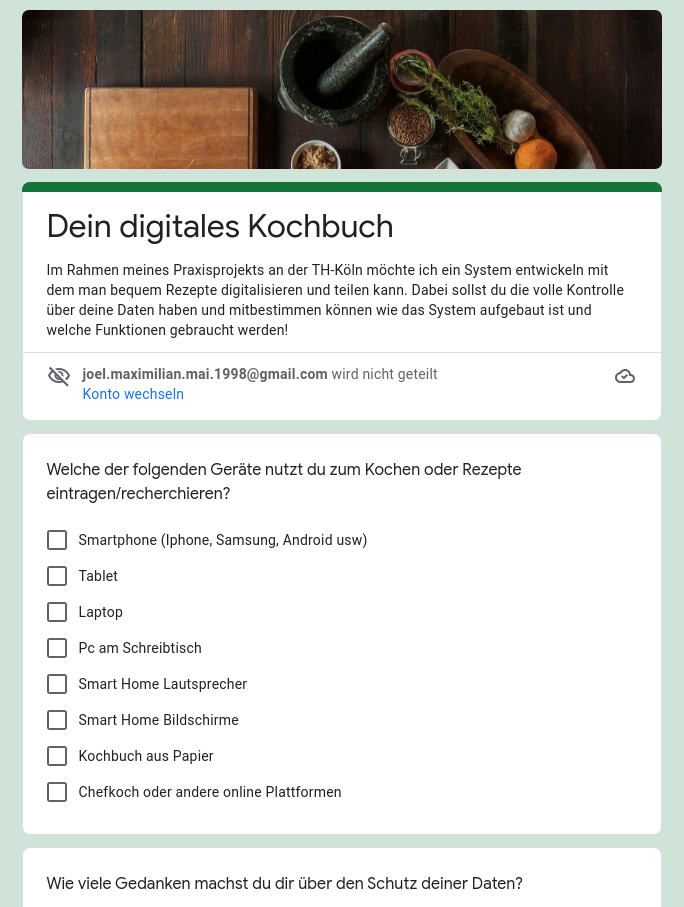
\includegraphics[width=0.3\textwidth]{images/umfrage.png}
  \centering
\caption[Google Formular (Ausschnitt)]{Google Formular (Ausschnitt)}
\label{fig:googleforms}
\end{wrapfigure}
Für die Stakeholder, die für die Priorisierung der Anforderungen interviewt worden sind, wurde aus möglichst jeder Zielgruppe zwei Personen in die Workshops eingeladen. Die Workshops bestanden aus einem Zoommeeting und einem Conceptboard Dienstes names Miro. Vor Beginn der Meetings wurden Karten angelegt welche die Erarbeitung der User Stories nach Jeff Patton\citep{Patton_2014} erläutern und zur Moderation beitrugen. Im Nachgang wurden die erarbeiteten User Stories priorisiert und umformuliert. \\
% Anzahl der Befragten und Mehr informationen zu den einzelnen Zielgruppen

\subsection{Verfahren zur Integration der menschzentrierten Gestaltungsaktivitäten}     
Für die Evaluierung der Gestaltungslösungen und ähnlichen Artefakten wie Wireframes und LowFideltyPrototypes wurden die selben und weitere Stakeholder über Googles Umfrage Tool interviewt um die Auswertung zu erleichtern. Dabei erhielten die Befragten vorgefertigte Antwortmöglichkeiten aber auch ein Freitext Forumular um etwaige persönliche Antworten zu geben. Die Auswertung der Formulare ergab dann Richtwerte für die Anordnungen von Elementen in den Gestaltungen aber beeinflusste auch die Entwicklung der Navigationmap.
% Konkrete Ergebnisse einbauen

\subsection{Projektplanung}
\begin{figure}[h] %!=overrides latex; h=here; t=top; b=bottom; p=special page for floating objects
    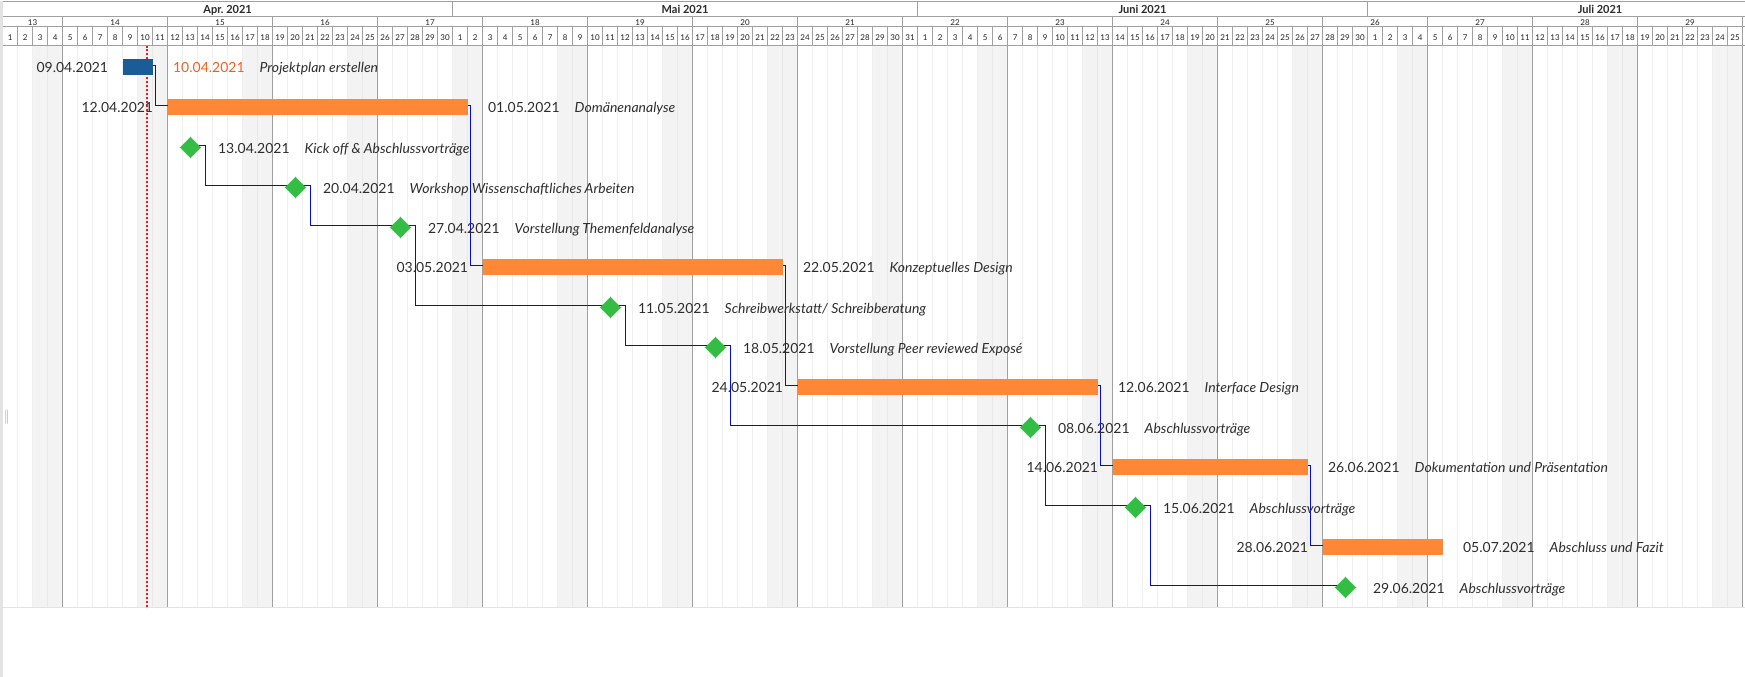
\includegraphics[width=1\textwidth]{images/ganttdiagramm.png}
    \caption[Ganttdiagramm]{Ganttdiagramm}
    \label{fig:ganttdiagramm}
\end{figure}
Um das Projekt möglichst transparent und nachvollziehbar zu gestalten wurden noch vor der Bearbeitung der Artefakte Tools und Workflows ausgewählt oder erarbeitet die den Aufwand an einzelnen Tasks und Features zu dokumentieren. Dabei wurde ein Dockercontainer eines Projektmanagementtools verwendet um grobe Projektphasen zu skizzieren, und eine Exceltabelle für die automatische Errechnung der Zeitaufwende nach Markdown exportiert um so in das \href{https://github.com/Inf166/PPSS21Mai/wiki}{Github Wiki} integriert zu werden. Im Github Wiki wurden die wesentlichen Erkenntnisse und die \href{https://github.com/Inf166/PPSS21Mai/wiki/Roadmap}{Roadmap} festegehalten die sich aus diesem Workflow ergaben.\\